% Author: Pavol Loffay
% Project: Master thesis - Hawkular alert prediction
% Date 20.2.2015

\documentclass[12pt,oneside]{fithesis2}
% Packages
\usepackage[english]{babel}       % Multilingual support
\usepackage[utf8]{inputenc}       % UTF-8 encoding
\usepackage[T1]{fontenc}          % T1 font encoding
\usepackage[scaled=0.86]{berasans}
\usepackage[scaled=1.03]{inconsolata}
\usepackage[plainpages = false,pdfpagelabels]{hyperref}

\usepackage{multicol}

% my declared packages
% Images
\usepackage{graphicx}
\usepackage{float} 
% Math
\usepackage{amsfonts}
\usepackage{amsthm}
\usepackage{amsmath}
\usepackage{commath} % abs
% Data structures, algorithms
\usepackage{listings}
\usepackage{algorithm} %algorithmix
\usepackage[]{algpseudocode} %noend
\lstset{language=java}

\usepackage{tabularx}
\usepackage{multirow}
\usepackage{pgf-pie}
%\definecolor{LightCyan}{rgb}{0.88,1,1}
%\usepackage{natbib} % for csplainnat.bib


% Url
\usepackage{url}
%\Urlmuskip=0mu plus 1mu
%\DeclareUrlCommand\url{\def\UrlLeft{<}\def\UrlRight{>} \urlstyle{tt}}

\usepackage{xparse}
\NewDocumentCommand{\INTERVALINNARDS}{ m m }{
    #1 {,} #2
}
\NewDocumentCommand{\interval}{ s m >{\SplitArgument{1}{,}}m m o }{
    \IfBooleanTF{#1}{
        \left#2 \INTERVALINNARDS #3 \right#4
    }{
        \IfValueTF{#5}{
            #5{#2} \INTERVALINNARDS #3 #5{#4}
        }{
            #2 \INTERVALINNARDS #3 #4
        }
    }
}

\newcommand{\ts}{\textsuperscript}
%\newcommand\nth{\textsuperscript{th}\xspace}

\hyphenation{data-bases}
\hyphenation{gar-bage}
\hyphenation{re-using}

\thesistitle{Alert Prediction in Metric Data Based on Time Series Analysis} % enter thesis title
\thesissubtitle{Master thesis}  
\thesisstudent{Bc. Pavol Loffay}    % name of the author
\thesiswoman{false}          % defines author’s gender  
\thesisfaculty{fi}  
\thesisyear{spring 2016}  
\thesisadvisor{RNDr. Adam Rambousek, Ph.D.} % fill in advisor’s name
\thesislang{en}                 % thesis is in English  

\begin{document}
\FrontMatter                    % The front matter
\ThesisTitlePage                % The title page
\begin{ThesisDeclaration}       % The declaration
  \DeclarationText
  \AdvisorName
\end{ThesisDeclaration}

\begin{ThesisThanks}            % The acknowledgements (optional)
  I would like to thank my supervisor RNDr. Adam Rambousek, Ph.D., Mgr. Jiri Kremser,
  family and the people from Hawkular team. Next, my thanks goes to Ing. Daniel Němec, Ph.D.
  for consulting theory behind time series analysis.

  Last but not least, I would like to thank to company Red Hat that provided me 
  with great opportunity to work on this project.
\end{ThesisThanks}

\begin{ThesisAbstract}          % The abstract
  The aim of the master's thesis is to develop a module for an open source monitoring
  and management platform Hawkular. This module is responsible for predicting
  alerts based on time series and providing data for predictive charts in Hawkular user interface.
\end{ThesisAbstract}

\begin{ThesisKeyWords}          % The keywords
  Time Series, Hawkular, Alert Prediction, Exponential Smoothing
\end{ThesisKeyWords}

\tableofcontents                % The table of contents
%   \listoftables                   % The list of tables (optional)
%   \listoffigures                  % The list of figures (optional)

\MainMatter                     % The main matter
% Author: Pavol Loffay
% Project: Master thesis - Hawkular alert prediction
% Date 20.2.2015

\chapter{Introduction}
In driving successful business on the internet it is important to assure an application
health and reliability. One can achieve that by monitoring subjected resources and setting
up a clever alerting system. These features are offered in many monitoring systems, however 
being predictive in this area can even prevent undesirable states and most importantly gives administrators more time for
reacting to such events. For instance it can decrease downtime of an application 
or ability to load balance workload in advance by horizontal scaling targeted services. 

As alerting system are sophisticated and can be composed by many conditions so this work
focuses only on predicting future metrics values which are then sent as input to an alerting system. 

In the first chapter are discussed various approaches for time series modeling and
forecasting. Second chapter focuses on implemented models with validation on real and 
generated test data sets. Implementation details with testing can be found in fourth chapter.

TODO describe chapters

    \section{Hawkular}
    The implementation part of the master's thesis is developed as a part of an open source project
    Hawkular\footnote{Available at \url{http://www.hawkular.org}}. 
    Therefore the application architecture and used technologies had to fit 
    into the overall project architecture.

    Hawkular is middleware monitoring and management platform
    developed by company Red Hat and independent community of contributors.
    It is a successor to very successful RHQ\footnote{Available at \url{https://rhq-project.github.io/rhq/}} 
    project, also known as JBoss Operations Network.
    By monitoring is meant that there are agents for diverse applications which
    push data to the server. These agents can also execute application specific actions. 

    The monolithic architecture of RHQ project was due it's size hard to maintain 
    and lacking robust REST API lead to fresh development of new application.   
    In contrast Hawkular consist of several loosely coupled or even independent applications.
    These independent components are much
    easier to maintain and more importantly they communicate over REST API. This
    architecture of microservices and chosen protocol allow simple development of 
    agents which can be written in any programming language. In RHQ only Java agent were
    available. Hawkular as product is customized Wildfly
    \footnote{An open source project of JBoss EnterpriseApplication Platform.}
    application server with all components deployed in it.

    \begin{itemize}
        \item Console\,--\,user web interface
        \item Accounts\,--\,authorization subsystem based on Keycloak\footnote{An open
            source single sing-on and identity management for RESTful web services.}
        \item Inventory\,--\,graph based registry of all entities in Hawkular
        \item Metrics\,--\,time series metrics engine based on Cassandra\footnote{An open
            source distributed database management system. Hybrid between key\,--\,value and
        column\,--\,oriented database.}
        \item Alerts\,--\,alerting subsystem based on JBoss Drools
    \end{itemize}

    Some of the modules uses also Java messaging topics (JMS) for inter\,--\,component
    one to many communication.

    Modules are packaged as standard Java web archives (WAR), or enterprise archives (EAR)
    and deployed into customized Wildfly. Build and package management is performed by 
    Maven and Gulp for user interface modules. 

    \section{Data Mining Goals}
    The goal of this thesis is to develop module for Hawkular which will provide forecasts for any 
    time series metrics collected by agent. On new metric data available the module
    learns from data and predicts new values. Based on this predicted values an alert can
    be triggered. Forecast should be also available for user interface in predictive
    charts. 

    One Wildfly agent on average collects hundreds to thousands metrics, therefore module
    should be capable of processing high volume of data. Some of the customers monitor
    hundreds of server each with multiple agents. Therefore performance of chosen 
    learning algorithm has to be taken in account.

%%%%%%%%%%%%%%%%%%%%%%%%%%%%%%%%%%%%%%%%%%%%%%%%%%%%%%%%%%%%%%%%%%% 
\chapter{Existing Solutions}
%TODO
TODO describe existing software.


%%%%%%%%%%%%%%%%%%%%%%%%%%%%%%%%%%%%%%%%%%%%%%%%%%%%%%%%%%%%%%%%%%% 
\chapter{Time Series Models}
This chapter focuses on time series theory and various approaches for modelling time series.
Models are ordered from simpler to more complex ones. 

Firstly, it is important to define time series; it is sequence of observations
$s_t \in \mathbb{R}$ ordered in time. This thesis focuses only on univariate equidistant 
discrete time series. Time series analysis contains many segments, this work focuses on 
forecasting. It is defined as a process of making prediction of the future based 
on the past. In other words, forecasting is possible because  
future depends on the past or analogously because there is a relationship
between the future and the past. However, this relation is not deterministic and 
can be hardly written in an analytical form.

There are two forecasting types: qualitative and quantitative.
Qualitative methods are mainly based on the opinion of the subject and are used 
when past data are not available, hence not suitable for this project. 
If there are past data available, quantitative forecasting methods are more suitable. 

TODO mention that we talk only about models which makes sense to use in our environment.

    %%%%%%%%
    \section{Simple quantitative methods}
    Following methods are the simples forecasting quantitative models. They can be used on
    any time series without further analysis. 

    \begin{itemize}
        \item Average method\,--\,forecasts are equal to the value of the mean of
            historical data.
            \begin{eqnarray}
                \hat{y}_{T+h|T} = \overline{y} = (y_{1}+ \dots + y_{T}) / T 
            \end{eqnarray}
        \item Na\"{i}ve method\,--\,forecasts are equal to the last observed value.
            \begin{eqnarray}
                \hat{y}_{T+h|T} = y_{T}
            \end{eqnarray}
        \item Drift method\,--\,variation of na\"{i}ve method which allow the
            forecasts to increase or decrease over time.
            \begin{eqnarray}
                \hat{y}_{T+h|T} = y_{T} + \frac{h}{T-1} \sum_{t=2}^T{y_{t} - y_{t-1}} = 
                    y_{T} + h(\frac{y_{T}-y_{1}}{T-1}) 
            \end{eqnarray}

    \end{itemize}
    There is also a seasonal variant of na\"{i}ve model. This method is suitable only
    for highly seasonal data. These methods in general produces high forecasting error 
    but are very easy to implement.

    %%%%%%%%
    \section{Linear Regression}
    Linear regression is classical statistical analysis technique. It is often used to
    determine whether there is linear relationship between dependent and eventually more
    independent variables. It is also often used for predictions mainly in econometric
    field. 

    Simple linear regression is defined as:
    \begin{eqnarray}
        y = \beta_0 + \beta_1 x + \epsilon
    \end{eqnarray}

    Parameters $\beta_0$ and $\beta_1$ are calculated by minimizing the sum of squared
    errors:
    
    \begin{eqnarray}
        SSE = \sum_{i=1}^N \epsilon_{i}^2 = \sum_{i=1}^N (y_i - \beta_0 - \beta_1 x_i)^2
    \end{eqnarray}
    
    Once parameters are estimated predictions for any time in the future can be calculated. 
    If modelled time series is not stationary then and for instance trend changes over
    time parameters has to be periodically estimated to achieve better accuracy. 
    %For econometric analysis it is important to use best linear unbiased estimator,
    %where couple of assumptions has to hold:
    %\begin{enumerate}
    %    \item $E(Y_i) = \beta_0 + \beta_1 X_i$
    %    \item $var(Y_i)=\sigma^2$\,--\,homoscedasticity
    %    \item $cov(Y_i, Y_j)=0$, for $i \neq j$
    %    \item $Y_i$ cames from normal distribution
    %    \item $X_i$ is not random variable
    %\end{enumerate}
    %Where $i$ takes values from $1$ to the number of observed values. These assumptions 

    %%%%%%%%
    \section{Simple Exponential Smoothing}
    The concept behind simple exponential smoothing is to attach 
    larger weights to the most recent observations than to observations from distant
    past. Forecasts are calculated using weighted averages where the weights 
    decrease exponentially as observations come from further in the past.
    In other words smaller weights are associated to older observations.
    Equation for simple exponential smoothing is listed in \ref{exp_smoothing}.

    \begin{eqnarray} \label{exp_smoothing}
         \hat{y}_{T+1|T} = l_t \\ \nonumber
         l_t = \alpha y_t + (1-\alpha)l_{t-1}
    \end{eqnarray}

    For smoothing parameter $\alpha$ holds $ 0 \leq \alpha \leq 1 $. Note, if $\alpha = 1$ then \\
    $\hat{y}_{T+1|T} = y_{T}$ so forecasts are equal to the na\"{i}ve method.
    If the parameter $\alpha $ is smaller more weight is given to observations from distance
    in past. 

    Simple exponential smoothing has flat forecast function, that means all forecasts
    all the same. Smoothing can be generally used as technique to separate signal and noise.
    This method is useful if a series does not contain any trend or one is interested only
    in one step ahead prediction. Multi step ahead predictions for time series with trend
    can produce high error.

    %%%%%%%%
    \section{Holt's Liner Trend Method}
    Simple exponential smoothing can be extended to allow forecasting of data with a trend. 
    This was done by Charles C. Holt in 1957. This method is slightly more complicated than 
    original one without trend. In order to add trend component another equation has to be added. 

    \begin{eqnarray} \label{exp_holt}
        \hat{y}_{t+h|t} = l_{t} + hb_{t} \\ \nonumber
         l_t = \alpha y_t + (1 - \alpha) (l_{t-1} + b_{t-1}) \\ \nonumber
         b_t = \beta (l_t - l_{t-1}) + (1 - \beta)b_{t-1} 
    \end{eqnarray}

    Where a parameter $b_t$ denotes a slope of the series and the parameter $l_t$ level. 
    There is also a new parameter smoothing parameter of the slope\,--\,$\beta$. 
    It's rage is equal to $\alpha$, so $\alpha,\beta \in \interval[{0,1}]$. 

    %%%%%%%%
    \section{Holt\,--\,Winters Seasonal Method}
    This method is an extension of Holt's linear trend method with added
    seasonality. It is also called triple exponential smoothing. In this model 
    there are three equations \ref{exp_holt_winters}. 
    One for level, second for trend and third for seasonality.
    Each pattern uses smoothing constant $ \alpha,\beta,\gamma \in \interval[{0,1}]$.

    \begin{eqnarray} \label{exp_holt_winters}
        \hat{y}_{t+h|t} = l_{t} + hb_{t} + s_{t+h_m-m}\\ \nonumber
        l_t = \alpha (y_t - s_{t-m}) + (1 - \alpha) (l_{t-1} + b_{t-1}) \\ \nonumber
        b_t = \beta (l_t - l_{t-1}) + (1 - \beta)b_{t-1} \\ \nonumber
        s_t = \gamma (y_t - l_{t-1} - b_{t-1}) + (1-\gamma)s_{t-m}
    \end{eqnarray}

    Where $h_m=[(h-1) \mod m] + 1$, which ensures that the estimates of the seasonal
    indices came from the correct season. This model can be used only if the period 
    of time series is know beforehand. In Hawkular the period of the time series is 
    unknown, therefore period identification should be also implemented.
    
    %%%%%%%%
    \section{Box\,--\,Jenkins Methodology (ARIMA)}
    Models from Box\,--\,Jenkins methodology are the most widely used in time series
    analysis specially for econometric data. This methodology is based on analysis of autocorrelation (ACF)
    and partial autocorrelation (PACF) functions.
    
    The most generic model is ARIMA(p, d, q). It combines together autoregressive, integrated and
    moving average models. An autoregressive model (AR) consist of sum of weighed lagged observations. It is listed
    in \ref{ar_model}. The order of this model is defined by $p$ and can be determined from PACF function \cite{cipra}.
    A moving average model (MA) is sum of weighted errors of order $q$. The order of this part can be
    determined from ACF function \cite{cipra}. The last part of the model is used when a time series is non stationary.
    There are several ways how to make a  particular time series stationary. Box Jenkins methodology uses
    differencing\,--\,integration part. The order if differencing original series is denoted by $d$ letter. Usually
    first order differences are enough to make time series stationary.

    Parameters of the model, including AR and MA part can by estimated by non-linear
    least squares or maximum likelyhood estimation \cite{brockwell}. For successful estimation a certain number of
    historical points needs to be available. In \cite{cipra} minimal training size is set to at least fifty
    observations.

    \begin{eqnarray} \label{ar_model}
        y_t = \phi_1 y_{t-1} + \phi_2 y_{t-2} + \dots + \phi_p y_{t-p} + \epsilon_t \\ \nonumber
        \epsilon_t \overset{iid}{\sim} N(0, \sigma^2)
    \end{eqnarray}

    Moving averages model should not be confused with simple moving average which is
    used for trend estimation. In moving average model MA(q) the current value is
    a regression against white noise of prior values of the series \cite{wiki-ma-model}. A random noise from
    each point is assumed to come from the same distribution which typically is 
    a normal distribution. Model of the order $q$ is listed in \ref{ma_model}.

    \begin{eqnarray} \label{ma_model}
        y_t = \theta_1 \epsilon_{t-1} + \theta_2 \epsilon_{t-2} + \dots + \theta_p y_{t-q} + \epsilon_t \\ \nonumber
        \epsilon_t \overset{iid}{\sim} N(0, \sigma^2)
    \end{eqnarray}

    It is important mention that models AR(p) and MA(q) are invertible.
    Therefore any stationary AR(p) model can be written as MA($\infty$) and with some assumptions
    vice versa \cite{brockwell}. ARIMA model is often written with backshift operator $By_t=y_{t-1}$.
    With this operator ARIMA(p, d, q) is listed in \ref{arima}. On the left side of the equation is AR(P) process
    and on the right MA(q).

    \begin{eqnarray} \label{arima}
        (1- \phi_1B - \dots - \phi_pB^p)(1-B)^d y_t = \\ \nonumber
         c + (1+\theta_1B+\dots+\theta_qB^q) \epsilon_t
    \end{eqnarray}

    After this theoretical part it is clear that ARIMA models are more complicated than family of moving averages.

    %%%%%%%%
    \section{Artificial Neural Networks}
    Recently a large number of successful applications using neural networks for time series modeling show that they
    can produce valuable results \cite{ann-forecasting-state-art}. There are several non trivial issues with
    determining the appropriate architecture of the network. This has to be taken into account because it can
    dramatically effect learning performance and forecasting accuracy \cite{ann-model-selecting}.
    Besides the problems with selecting right architecture learning process of artificial neural network is much more
    computationally expensive than selecting appropriate ARIMA or exponential smoothing model \cite{ann-forecasting}.

    Because Hawkular forecasting engine should be capable of predicting thousands of metrics at the same time, models
    based on neural networks would have too high computational requirements. Therefore they are not suitable for our
    environment.

    %%%%%%%%
    %\section{Adaptive Filtering}
    %TODO probably I will delete this and discuss it in the conclusion that adaptive filtering can be used e.g. LMS
    %filter.

    %%%%%%%%
    \section{Time series decomposition}
    In modelling time series it is sometimes necessary to decompose series to trend, seasonal and random component
    \cite{otexts}. It is also used for initialization seasonal indices in triple exponential smoothing.

    \begin{itemize}
        \item \textbf{Trend $ T_{t} $}\,--\,exists if there is long term increase or decrease over
            time. Can be linear or nonlinear (e.g. exponential growth)
        \item \textbf{Seasonal $ S_{t} $}\,--\,exists when a series is influenced by seasonal factors.
            Seasonality is always of fixed and known period.
        \item \textbf{Cyclic $ C_{t} $}\,--\,exists it there are long term wave-like patterns.
            Waves are not of a fixed period.
        \item \textbf{Irregular $ E_{t} $}\,--\,unpredictable random value referred as white
            noise. 
    \end{itemize}

    Decomposition can be written in many forms. Two of them are additive and multiplicative \ref{decomposition}.
    Which one to use depends on the underlying time series model.

    \begin{eqnarray} \label{decomposition}
        y_{t} = T_{t} + S_{t} + C_{t} + E_{t} \\
        y_{t} = T_{t} \times S_{t} \times C_{t} \times E_{t}
    \end{eqnarray}

    An algorithm for additive decomposition consist of following steps:

    \begin{itemize}
        \item Compute a trend component $\hat{T}_t$ using moving average model. If a period is even use
        $2 x MA(period)$. If period is an odd number use $MA(period)$. $2 x MA$ for even period is used because it
        has to be symmetric.
        \item Calculate detrended series $y_t - \hat{T}_t$.
        \item Estimate seasonal indices $\hat{S}_t$ for each period by averaging values of given period. For example,
         the seasonal index for Monday is the average for all detrended Monday values in the data. Then the mean of
         seasonal indices is subtracted from each period.
        \item Random component is calculated by subtracting trend and seasonal component from original time series
            $\hat{E}_t = y_t - \hat{T}_t - \hat{S}_t$.
    \end{itemize}

    %%%%%%%%
    \section{Augmented Dickey\,--\,Fuller Test}
    Time series statistical tests are often used for testing if there is particular characteristics present in time
    series. Unit root test are used whether a time series in non stationary. In this work Augmented Dickey\,--\,
    Fuller (ADF) test was chosen for unit root testing. It's null hypothesis $H_0$ is time series contains a
    unit root \,--\, it is not stationary. Outcome of this test is a negative ADF statistics. The more negative it is
    the stronger the rejection of the hypothesis. The full form of ADF test is listen in \ref{adf-test}.

    \begin{eqnarray} \label{adf-test}
        \Delta y_t = \alpha + \beta t + \gamma \Delta y_{t-1} + \dots + \delta{p-1} \Delta y_{t-p+1} + \epsilon_t \\
        ADF = \frac{\hat{\gamma}}{SE(\hat{\gamma})} \label{adf-stat}
    \end{eqnarray}

    There are multiple variants of ADF test. Some of them leave out some parts of equation \ref{adf-test}.
    The most important ones and widely used are:

    \begin{itemize}
        \item \emph{nc}\,--\,no constant - for regression with no constant not time trend ($\beta t$)
        \item \emph{c}\,--\,constant for regression with an intercept but no time trend ($\beta t$)
        \item \emph{ct}\,--\,for a regression with an intercept and time trend
    \end{itemize}

    Each of them is good for testing particular type of stationarity. For example for testing if there is time trend
    present in the time series \emph{c} version is best choice.

    The implementation of this test is to fit multiple linear regression model of equation \ref{adf-test}. Then
    calculate ADF statistics with \ref{adf-stat}. SE denotes standard error of estimated $\hat{\gamma}$.

    %%%%%%%%
    \section{Seasonality detection}
    Forecasting engine in Hawkular system does not have any inside information of period of a time series being
    modelled. Therefore automatic period identification has to be implemented. In practice it is
    a difficult task and result often differs from correct period, specially if there is significant noise present in
    the series \cite{period-meteo}.

    There are several ways how to implement automatic period identification. The most used ones are based on
    autocorrelation function (ACF) or spectral density \cite{period-hydman}. This work applies ACF method.
    In the following chart \ref{img:period-acf} ACF function of sine function is shown. The period of this
    function is seven. There are patterns repeated every seven observations and it is decreasing to zero.

    \begin{figure}[H]
        \begin{center}
            \scalebox{0.5}{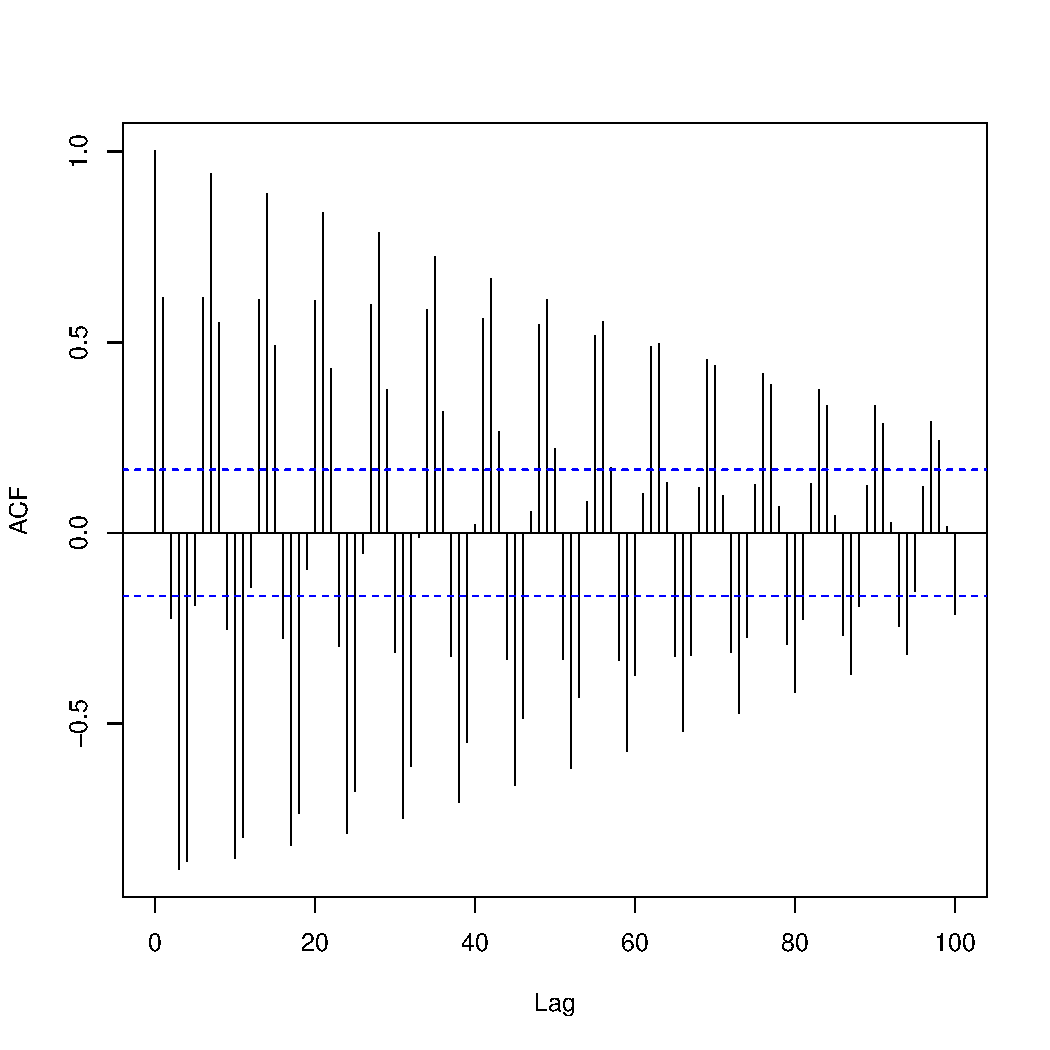
\includegraphics{img/acf-sine.pdf}}
            \caption{ACF of sine function.}
            \label{img:period-acf}
        \end{center}
    \end{figure}

    The algorithm for automatic period identification is demonstrated in \ref{alg:period-find}. It uses ACF function
    It is looking for periodically significant values of ACF function. These values have to be decreasing to zero at
    some rate. At the infinity lag ACF approach zero.

    The algorithm first calculates autocorrelation function of input time series and it finds index of the highest
    value. Follows \texttt{checkPeriodExists} where it checks if there are significant values of ACF present at following $n*period$
    indices of autocorrelation function. There have to be present at lease two consecutive values of ACF, so $n$ takes
    values from $1,2,3\dots$

    \begin{algorithm}
        \caption{Find period of time series} \label{alg:period-find}
        \begin{algorithmic}[1]
        \Function{findFrequency}{$int[] ts$}
            \If{$unitRootPresent(ts)$} \Comment{e.g. ADF test}
                \State $ts \gets diff(ts)$ \Comment{first order differences}
            \EndIf
            \State $acf \gets acf(ts)$ \\
                        \Comment{returns index of the highest value}
            \State $period \gets findHighest(ts, period)$
            \While{$period * 2 < ts.length$}
                \If{$checkPeriodExists(x, ts)$}
                    \State \Return $period$
                \EndIf
                $period \gets findHighest(ts, period)$
            \EndWhile
            \State \Return $0$
        \EndFunction
        \end{algorithmic}
    \end{algorithm}

%%%%%%%%%%%%%%%%%%%%%%%%%%%%%%%%%%%%%%%%%%%%%%%%%%%%%%%%%%%%%%%%%%%
\chapter{Models on Real Data}
In the previous chapter several models for forecasting were discussed, however in Hawkular only a few of them were
selected and implemented. It is because various time complexity of the models and more important robustness in terms of
beeing able to produce accurate results for higher range of modelled time series.
Following model evaluations and graphs are generated using statistical system R.

    %%%%%%%%
    \section{Metrics in Hawkular}
    In Hawkular there are three types of metrics: gauge, counter and availability. All of them are univariate metrics
    of structure $ \{timestamp, value\} $. Each of these types is used for collecting dedicated types of metric data.
    For example gauge can increase or decrease over the time, counter is monotonically decreasing or increasing and
    availability represents up or down state of a resource.

    %%%%%%%%
    \section{Evaluating Forecasting Accuracy}
    In order to evaluate model it is important to estimate an error of the forecast. There are 
    several statistics for evaluating forecasting errors. The most used ones are mean squared error (MSE)
    \ref{accuracy-mse} and mean absolute error (MAE) \ref{accuracy-mae}. The difference between them is that MSE
    emphasizes the extremes while MAE is more robust to outliers.

    \begin{subequations} \label{accuracy}
        \begin{align} \label{accuracy-mse}
             MSE = \frac{1}{n} \sum_{i=1}^{n}(y_i - \hat{y_i}) \\ \label{accuracy-mae}
             MAE = \frac{1}{n} \sum_{i=1}^{n} \abs{y_i - \hat{y_i}}
         \end{align}
    \end{subequations}

    %%%%%%%%
    \section{Model Selection}
    When comparing multiple models, statistics like MSE or MAE are not the best objective functions. Comparison
    based on this statistics can select complicated model with lots of parameters, which may overfits training data
    and most importantly it selects less robust model \cite{cipra}. Therefore for comparing multiple models another
    factors has to be added to objective function. These factors are number of parameters of the model. The
    most used criteria for model sections are: Akaike information criterion (AIC) and Bayesian information
    criterion (BIC). Model with lower information criterion is preferred.

    \begin{eqnarray} \label{aic}
        AIC = 2 k - \ln(L) \\ \nonumber
        BIC = k \ln(n) - 2 \ln(L)
    \end{eqnarray}

    Equations for AIC and BIC are listed in \ref{aic}. Number of parameters of the model represents $k$, $n$ is number
    of observations and $L$ is maximized value of the likelihood function of the model. In case for exponential
    smoothing it is minimized sum of squared error of one step ahead prediction of training data set. From the
    equations it can be seen that BIC penalizes models with more parameters. There is also AIC criterion with
    correction form \ref{aicc}. Corrected version of AIC more penalizes longer models.

    \begin{eqnarray} \label{aicc}
        AICc = AIC + \frac{2k(k+1)}{n-k-1}
    \end{eqnarray}

    %%%%%%%%
    \section{Evaluation on Data}
    Show graphs of models for sample time series.

%%%%%%%%%%%%%%%%%%%%%%%%%%%%%%%%%%%%%%%%%%%%%%%%%%%%%%%%%%%%%%%%%%% 
\chapter{Design and Implementation}
Module for an alert prediction was named Hawkular Data mining. Source
code\footnote{Available at \url{https://github.com/hawkular/hawkular-datamining}} is versioned in Git
hosted on Github. On every commit a build with integration and unit tests was triggered in
Travis CI. Pull requests were always reviewed by some team member.

In the following chapters is described integration, design and the most important
sections of implementation.

    %%%%%%%%
    \section{Integration with Hawkular}  
    Data mining module had to follow architecture of the whole Hawkular application.
    The same approach was followed as in other modules. That means the module 
    works also in standalone fashion without Hawkular. The build produces two Java
    web applications packaged as WAR. One is for standalone usage and other with
    integration code for Hawkular.

    Integration with Hawkular is showed in \ref{img_integration}.
    The module interacts with Inventory, Metrics and Alerts. User interface uses Data
    mining REST API for getting predictions for charts. Communication is done through 
    Java messaging system and REST calls. Therefore modules are
    loosely coupled.

    Metrics definitions and prediction metadata are stored in Inventory.
    Communication flows through JMS request response temporary queues. This was
    implemented specially for asking data across all tenants.

    Forecasting of 
    metrics in Hawkular is enabled by creating relationship from tenant to tenant, metric type
    or directly to metric in Inventory. Lower levels overrides higher (configuration on metric overrides
    configuration on metric type or tenant\dots). Every change in Inventory is sent to bus topic
    where other modules can consume it. When prediction gets enabled Data mining queries all
    historical metrics to initialize model.

    When Metrics receives data from Agent it sends them to topic where is consumed by Alerts
    and Data mining. If metric if being forecasting model weight are updated and predicted
    values are sent to the same topic. Original and predicted time series are consumed by 
    Alerts and conditions are evaluated. At this point an alert can be fired. 

    \begin{figure}[H]
        \begin{center}
            %TODO change to UML component diagram
            \scalebox{0.5}{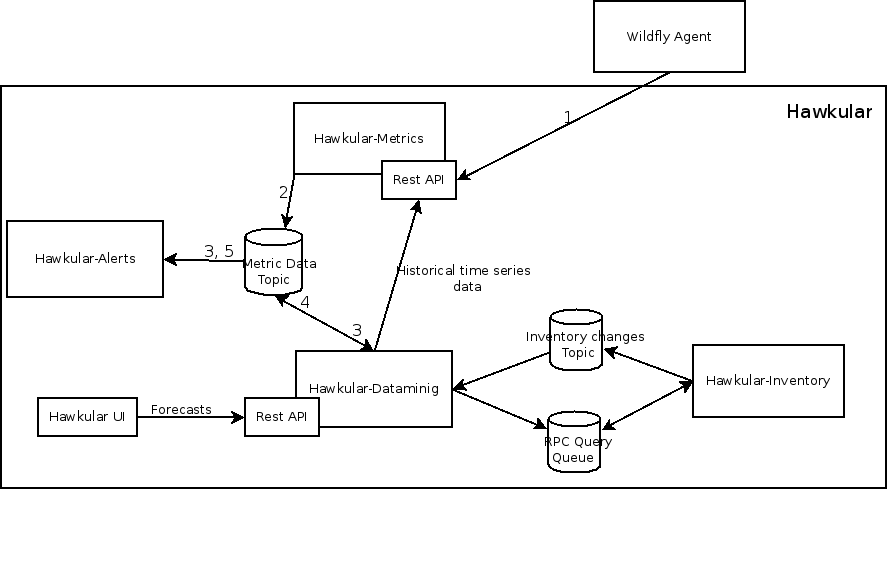
\includegraphics{img/architecture.png}} 
            \caption{The integration with Hawkular.}
            \label{img_integration}
        \end{center}
    \end{figure}

    %%%%%%%%
    \section{Design of Data Structures}
    In this section are described the most interesting parts of the implementation.
    
    Hawkular Inventory stores all entities of the application. Back end is graph
    database\footnote{Compatible with Apache Tinkerpop\,--\,Titan and TinkerGraph}.
    In the \ref{img_inventory} is showed part of the entities which are important for 
    Data mining module.
    Intentory high level API offers creating relationships between arbitrary entities. 
    This was used for enabling forecasting. This relationship contains properties map
    where is stored configuration of forecasting.

    \begin{figure}[H]
        \begin{center}
            \scalebox{0.5}{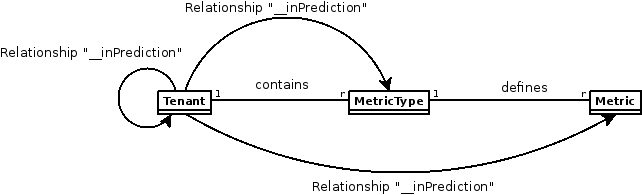
\includegraphics{img/inventory.png}} 
            \caption{Structure of Inventory.}
            \label{img_inventory}
        \end{center}
    \end{figure}

    For subscribing predictions and holding models was designed interface
    \texttt{ModelManager} \ref{alg_modelManager}. 
    Implementation of this interface holds in memory 
    objects of models with respect to hierarchy of Inventory.

    \begin{lstlisting}[caption={Interface Model Manager}, language=Java, label={alg_modelManager}]
     public interface ModelManager {
         void subscribe(Metric, Set<ModelOwner>);
         void unSubscribe(tenantId, metricId);
         Model model(tenantId, metricId);
         ...
     }
    \end{lstlisting}

    \texttt{ModelManager} is initialized on application startup and any change in
    Inventory is propagated through JMS to this object. With this approach Data mining is
    always synchronized with inventory. 

    Interface \texttt{ForecastingEngine} \ref{alg_forecaEngine} provides forecasts for
    subscribed metrics. Implementation of this interface contains \texttt{ModelManager}.
    
    \begin{lstlisting}[caption={Interface Forecasting Engine}, language=Java, label={alg_forecaEngine}]
     public interface ForecastingEngine {
         void learn(List<DataPoint> ts);
         void List<DataPoint> predict(tenantId, metricId, nAhead);
         ...
     }
    \end{lstlisting}

    \subsection{Automatic Forecaster}
        TODO

    \section{Model Optimization}


    %%%%%%%%
    \section{Tests Automation and Documentation}
    Unit tests were developed to cover crucial functionality of the program. The
    frameworks JUnit and TestNG are used for testing. Data mining module interacts with many other modules so
    integration and end to end tests were also implemented. Integration and end to end
    tests were written in Groovy because of the simple and well-arranged http client. It
    is also possible to easy define JSON string which is sent as POST object.

    Documentation is written directly in Java code as javadoc. Documentation of the REST
    API was automatically generated by framework Swagger\footnote{Available at
    \url{http://swagger.io/}} and then automatically uploaded at Hawkular website. This
    was done at every build in Travis-CI. With this approach there were always the newest 
    documentation available.

%%%%%%%%%%%%%%%%%%%%%%%%%%%%%%%%%%%%%%%%%%%%%%%%%%%%%%%%%%%%%%%%%%% 
\chapter{Evaluation of Implemented Models}
%TODO
TODO Do an example how to generate an alert.

    %%%%%%%%
    \section{Prediction capabilities}
    Show prediction capabilities of implemented models.
    TODO Can I compare it against R implementation?

    %%%%%%%% 
    \section{The Most Important Metrics}
    %TODO 
    TODO select subset of the most important metrics and show on them predictions.

%%%%%%%%%%%%%%%%%%%%%%%%%%%%%%%%%%%%%%%%%%%%%%%%%%%%%%%%%%%%%%%%%%% 
\chapter{Conclusion}


    
% Bibliography goes here
% Index goes here (optional)
\bibliographystyle{czplain}
%\bibliographystyle{csplainnat}
%\bibliographystyle{czechiso} % sets plain bibliography style
\bibliography{bibliography}     % BibTeX database file

% Appendix
\appendix
\chapter{Diagrams}
    \begin{figure}[H]
        \begin{center}
            % original from idea
            %\scalebox{0.34}[0.475]{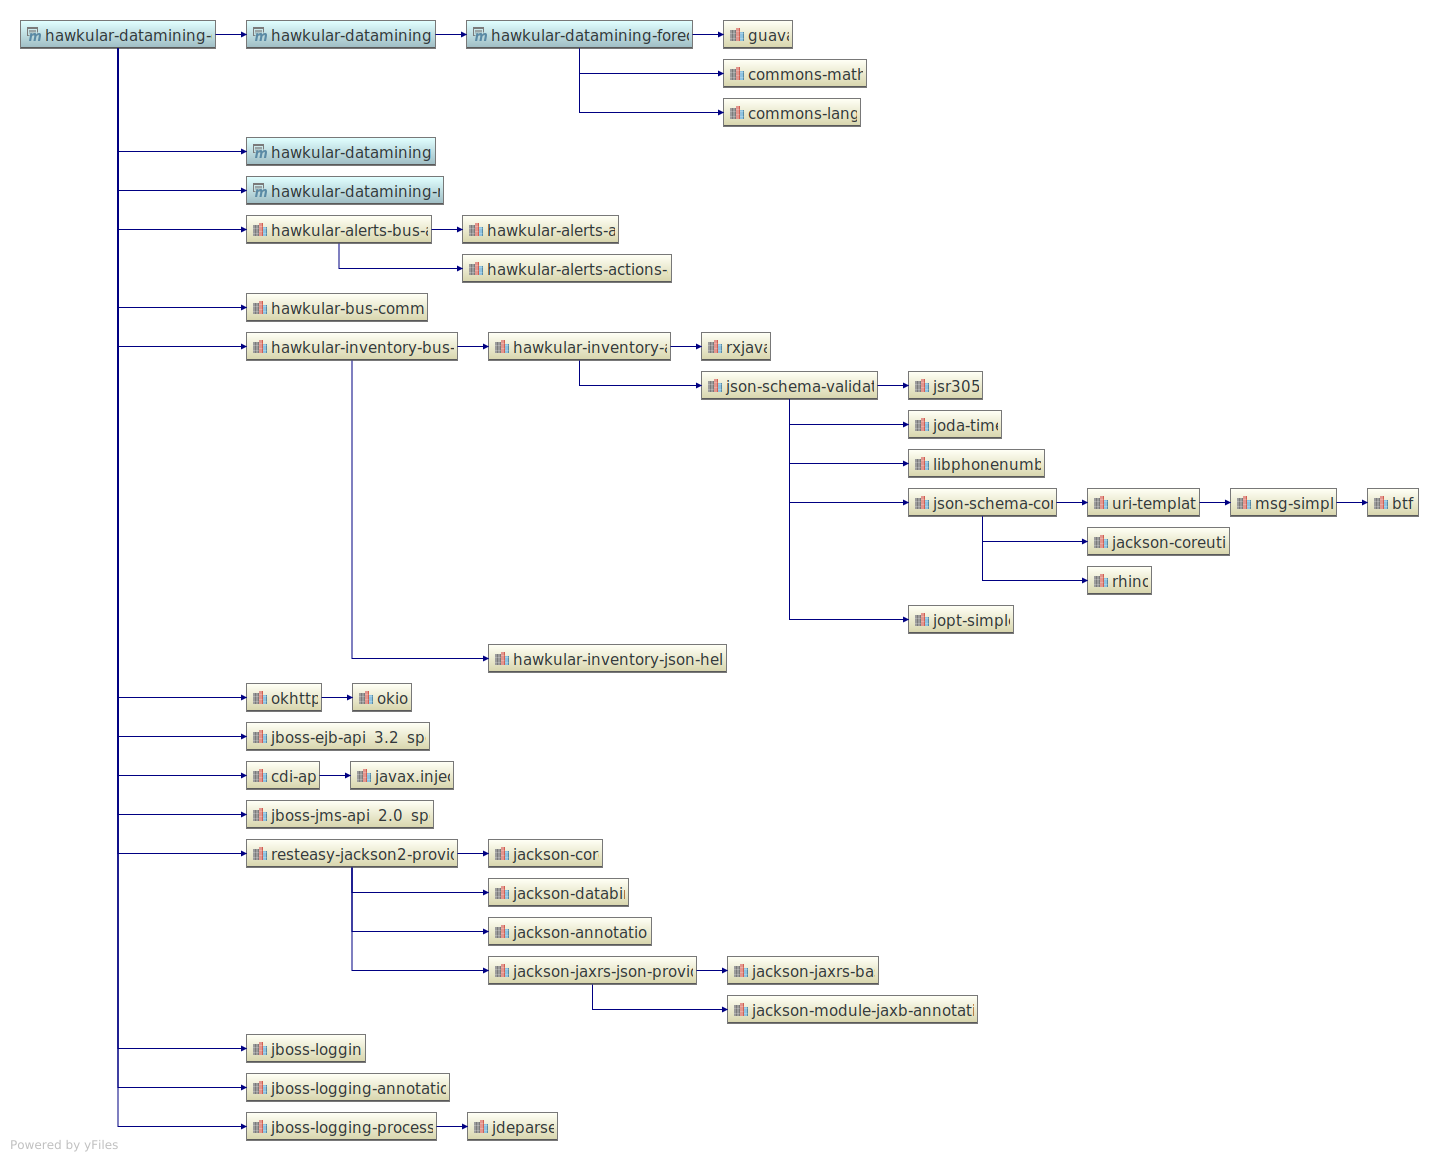
\includegraphics{img/src/maven-deps-tree.pdf}}
            \scalebox{0.6}{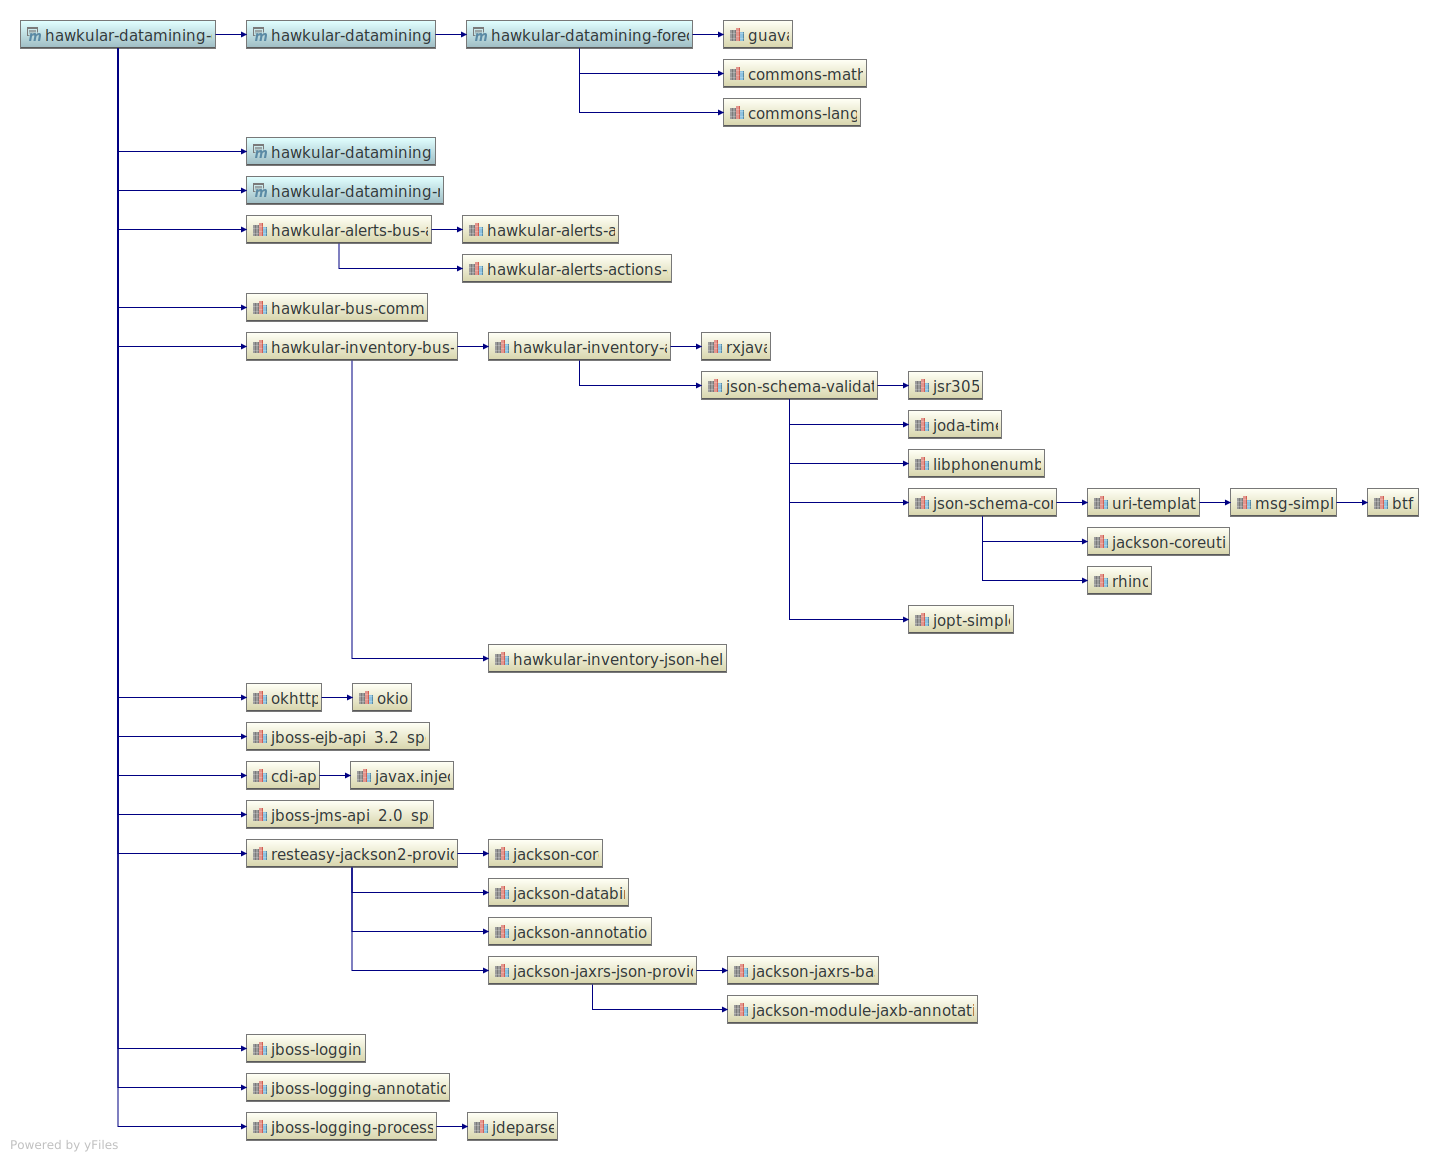
\includegraphics{img/src/maven-deps-tree.pdf}}
            \caption{Dependency tree of maven artifacts.}
            \label{appen:maven-deps}
        \end{center}
    \end{figure}

    \begin{figure}[H]
        \begin{center}
            \scalebox{0.35}[0.21]{\includegraphics[angle=90]{img/src/class-diagram.pdf}}
            \caption{Partial class diagram of \texttt{datamining-forecast} and \texttt{datamining-api}.}
            \label{appen:class-diagram}
        \end{center}
    \end{figure}

\chapter{Predictive Charts}
    \begin{figure}[H]
        \begin{center}
            \scalebox{0.6}[0.443]{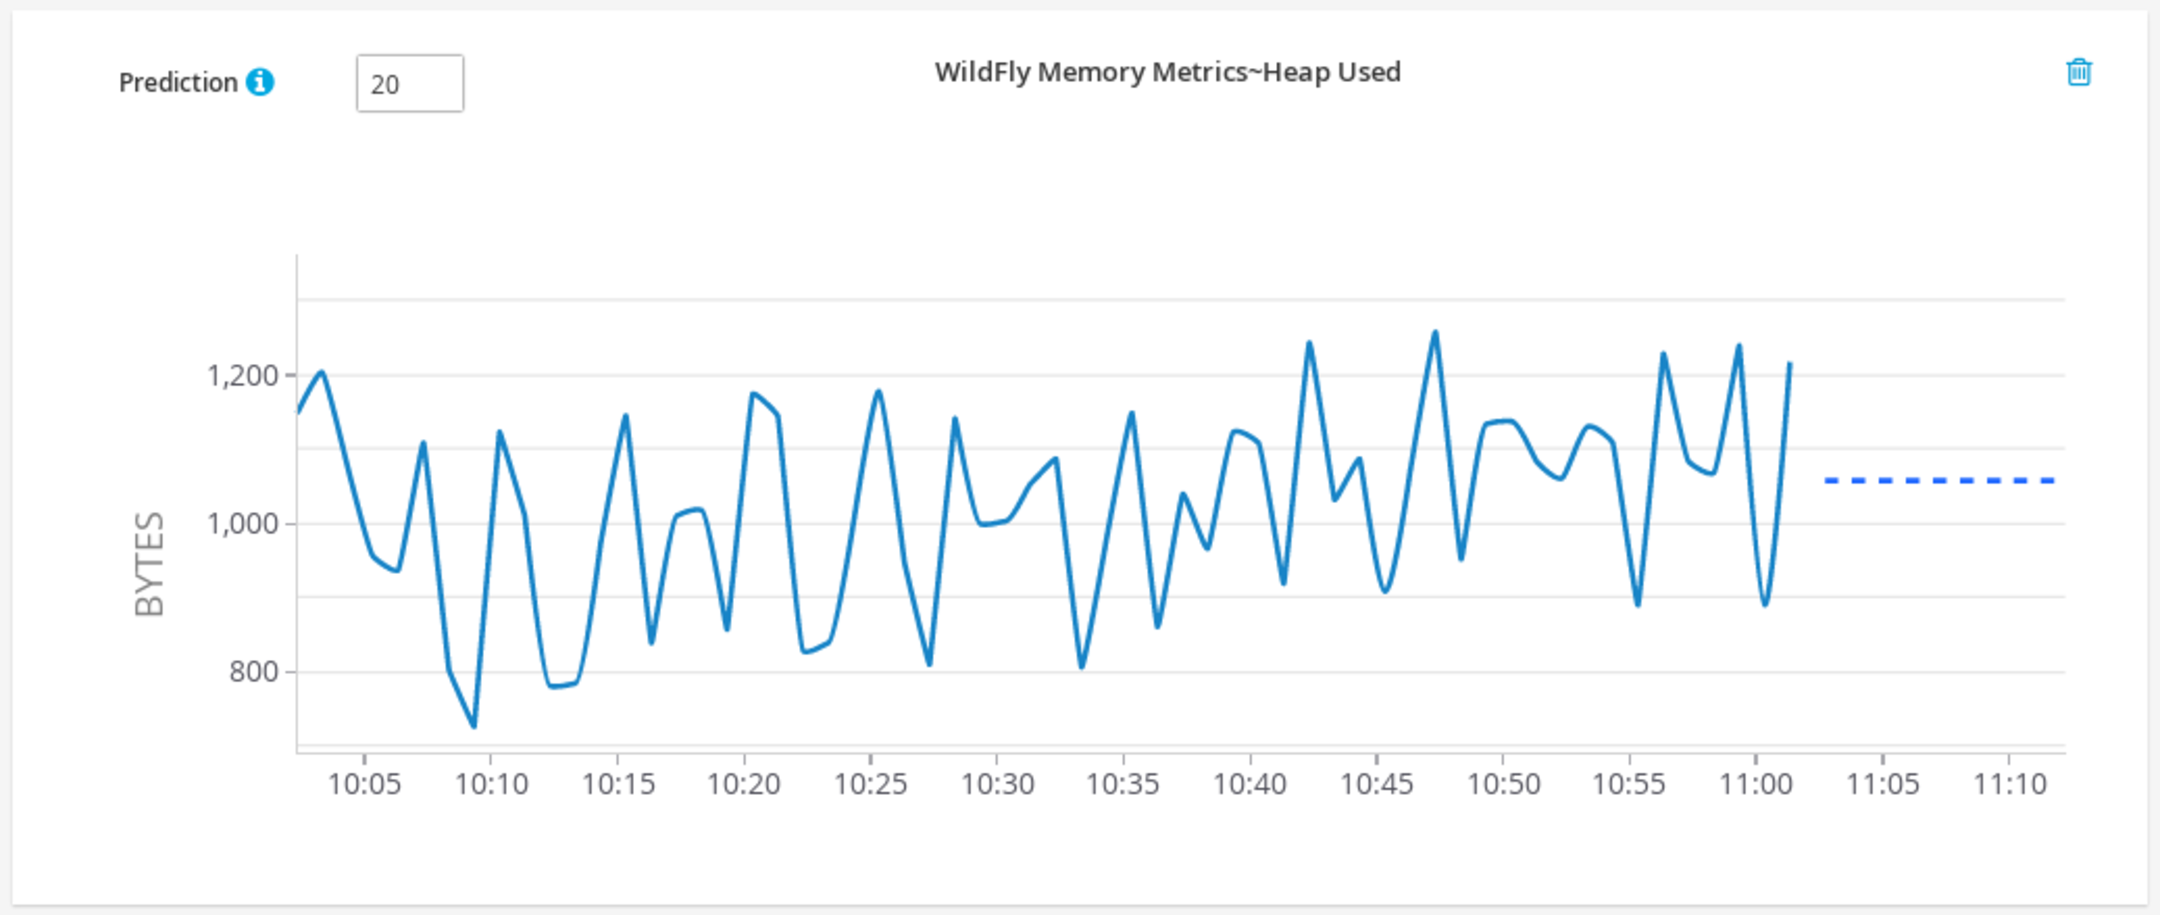
\includegraphics[angle=90]{img/hawkular-simple.pdf}}
            \caption{Predictive chart for simple exponential smoothing.}
            \label{appen:hawkular-simple}
        \end{center}
    \end{figure}
    \begin{figure}[H]
        \begin{center}
            \scalebox{0.6}[0.5]{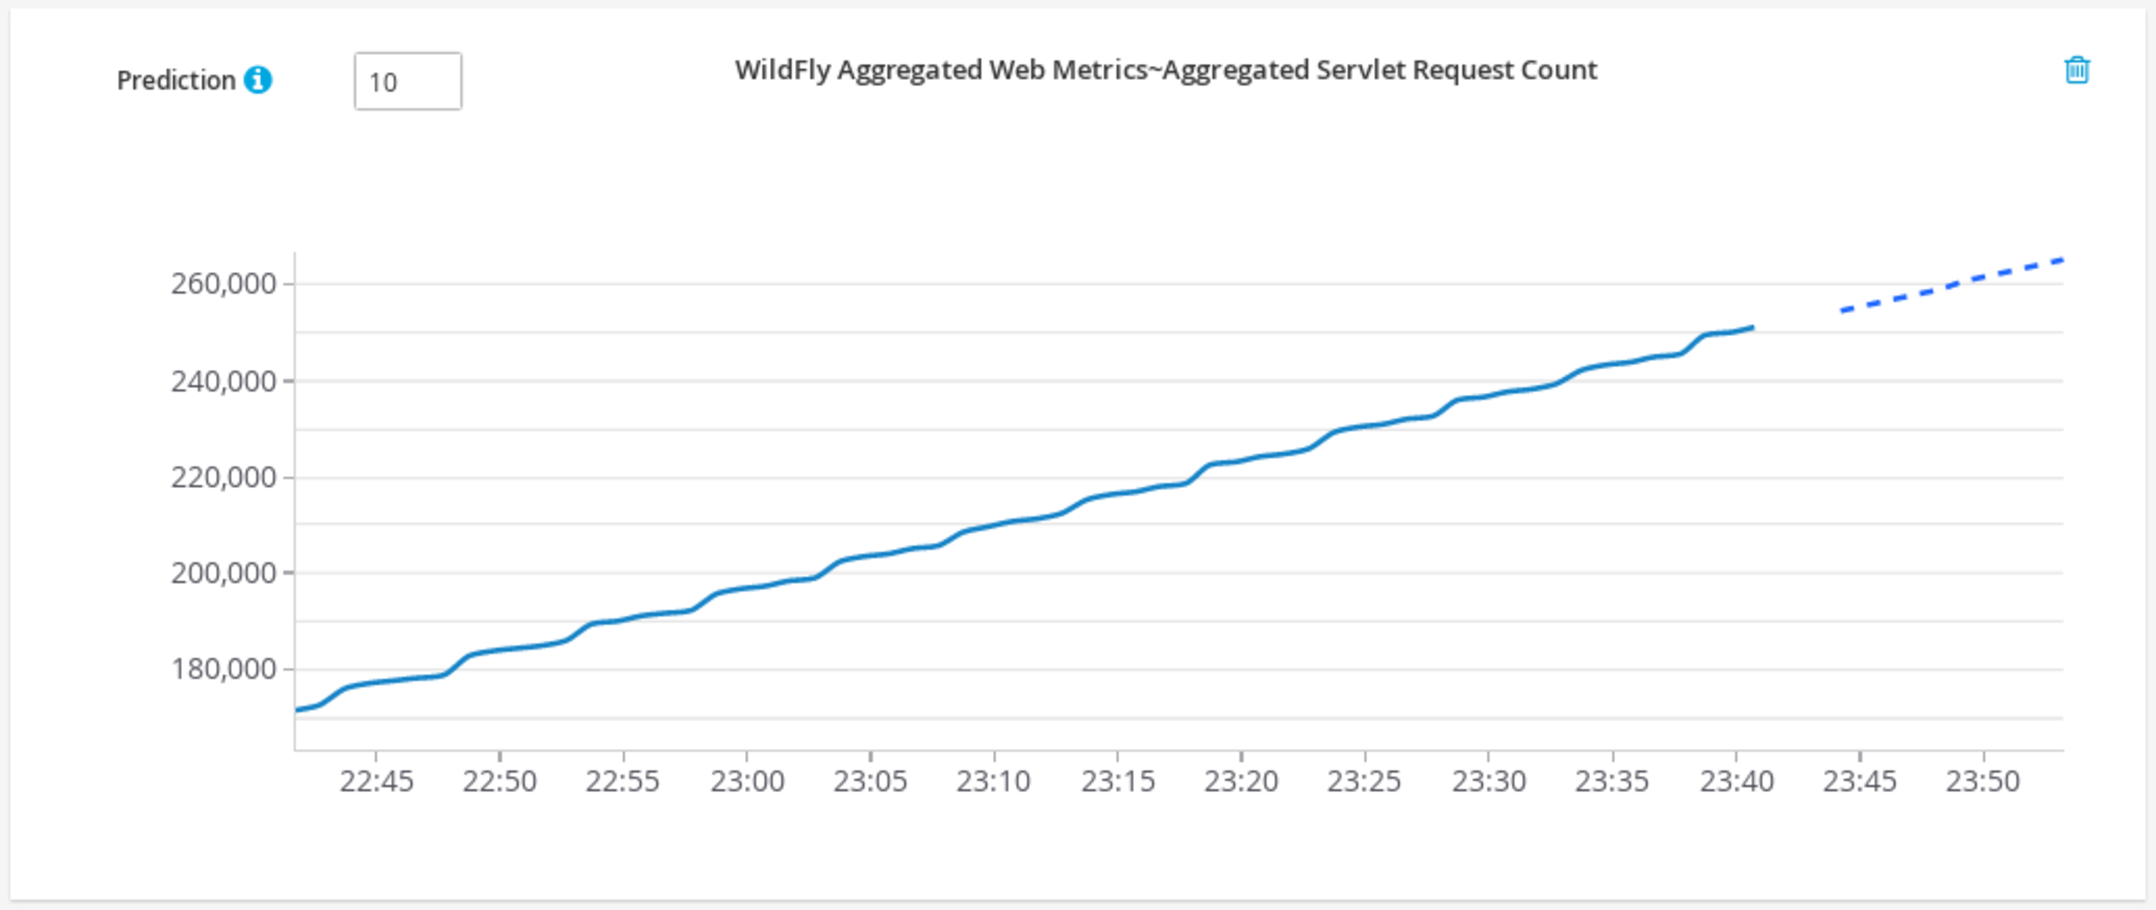
\includegraphics[angle=90]{img/hawkular-double.pdf}}
            \caption{Predictive chart for double exponential smoothing.}
            \label{appen:hawkular-double}
        \end{center}
    \end{figure}
    \begin{figure}[H]
        \begin{center}
            \scalebox{0.6}[0.5]{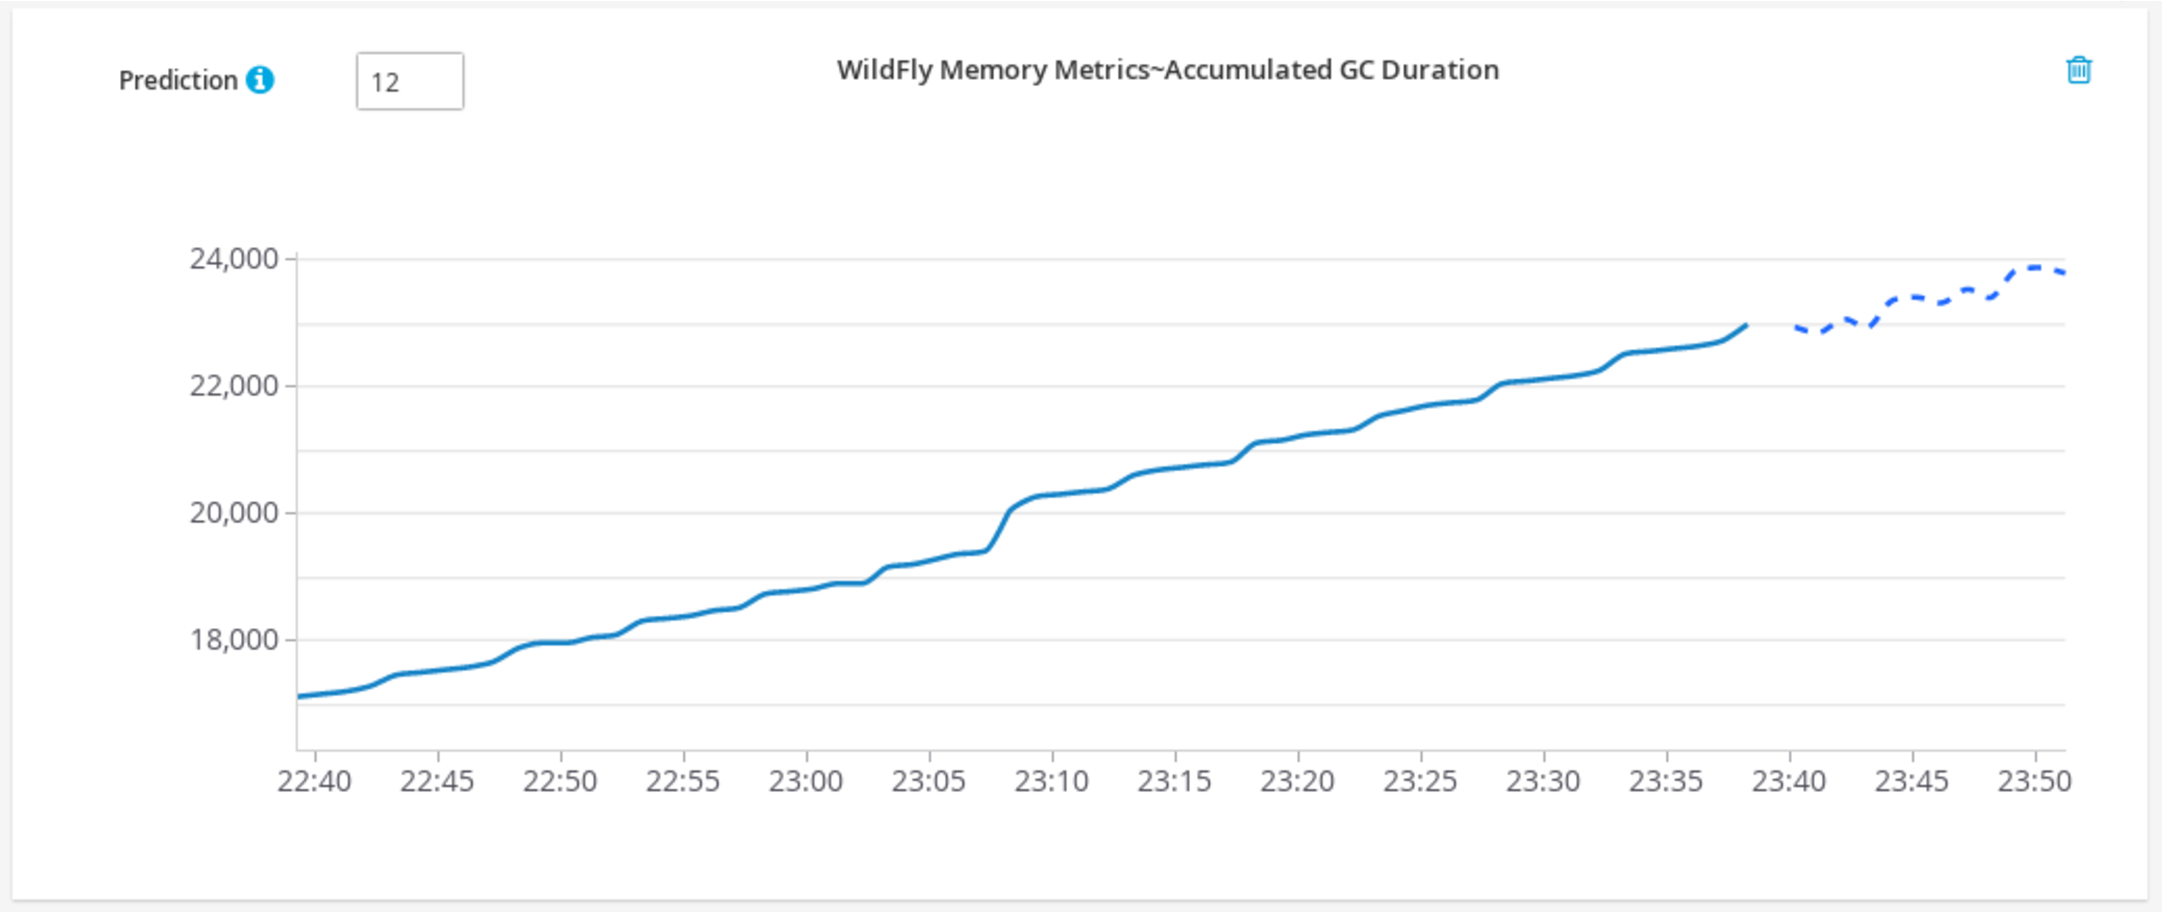
\includegraphics[angle=90]{img/hawkular-triple.pdf}}
            \caption{Predictive chart for triple exponential smoothing.}
            \label{appen:hawkular-triple}
        \end{center}
    \end{figure}

\chapter{Testing Time Series Samples} \label{appen:testing-samples}
    \begin{figure}[H]
        \begin{center}
            \scalebox{0.22}[0.62]{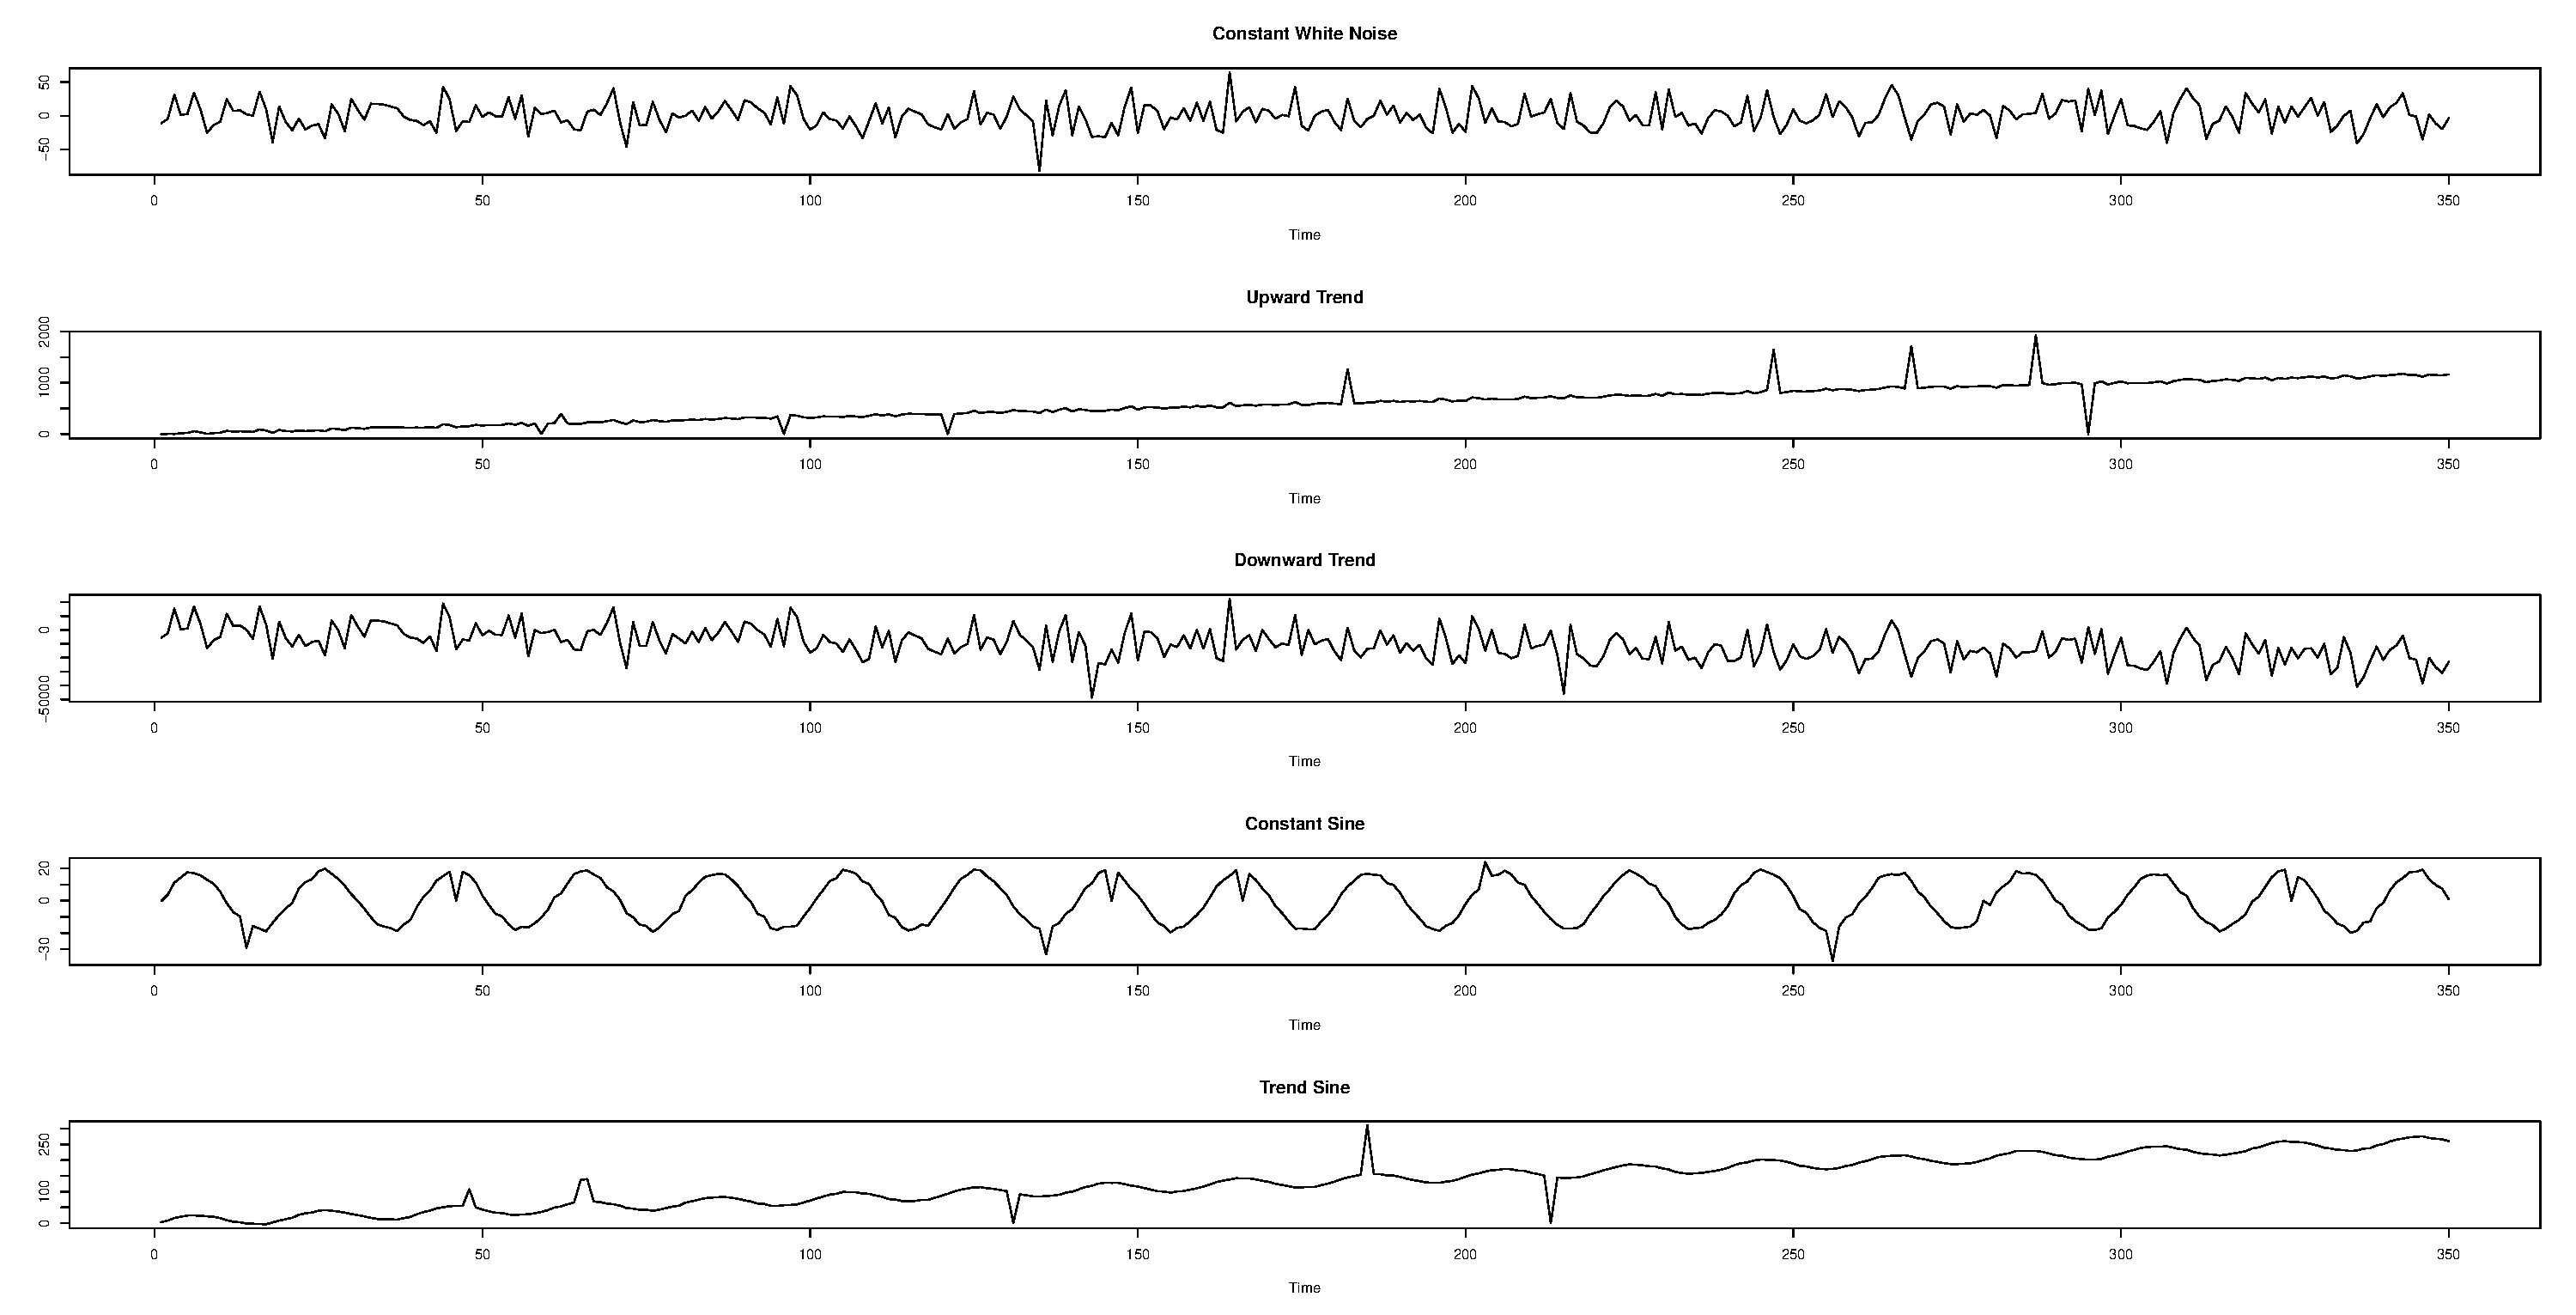
\includegraphics[angle=0]{img/testing-time-series.pdf}}
            \caption{Time series samples for evaluation.}
            \label{appen:img-testing-samples}
        \end{center}
    \end{figure}

\chapter{Tests Results} \label{appen:chap:results}

    \begin{table}[h]
        \begin{center}
            \begin{tabular}{c|c|c|c|c|c}
                \textbf{Test case} &
                \rotatebox{90}{wn} &  \rotatebox{90}{\texttt{trendUpLow}} & \rotatebox{90}{\texttt{trendDownHigh}} &
                \rotatebox{90}{\texttt{sine}} & \rotatebox{90}{\texttt{sineTrend}} \\ \hline \hline
                \multirow{2}{*}{48\,--\,12 (1)}   & 252.60 & 4293.10 & 59074630.35 & 19.91 & 291.89 \\
                                                  & 251.72 & 4602.83 & 57931198.55 & 19.97 & 291.90 \\ \hline
                \multirow{2}{*}{100\,--\,12 (1)}  & 247.72 & 702.52  & 117983966.67 & 23.54 & 25.82 \\
                                                  & 252.96 & 513.46 & 124329179.62 & 23.54 & 26.30 \\ \hline
                \multirow{2}{*}{200\,--\,12 (1)}  & 380.51 & 862.58 & 100868036.49 & 45.14 & 50.91 \\
                                                  & 380.57 & 718.39 & 101969913.50 & 45.14 & 47.95 \\ \hline \hline

                \multirow{2}{*}{48\,--\,12 (6)}   & 333.07 & 7071.66 & 90579713.93 & 483.70 & 1772.85\\
                                                  & 325.33 & 7206.03 & 89687108.81 & 483.88 & 1772.86 \\ \hline
                \multirow{2}{*}{100\,--\,12 (6)}  & 287.00 & 1916.31 & 125727085.38 & 420.33 & 346.06 \\
                                                  & 289.63 & 1531.48 & 130162180.73 & 420.33 & 347.18 \\ \hline
                \multirow{2}{*}{200\,--\,12 (6)}  & 325.67 & 1457.51 & 172882341.31 & 394.90 & 2734.56 \\
                                                  & 327.13 & 1132.87 & 172309610.96 & 394.90 & 2733.64 \\ \hline \hline

                \multirow{2}{*}{48\,--\,12 (12)}  & 271.78 & 7556.76 & 71166890.64 & 535.57 & 2956.52 \\
                                                  & 276.16 & 7742.00 & 71094737.26 & 535.46 & 2956.52 \\ \hline
                \multirow{2}{*}{100\,--\,12 (12)} & 239.68 & 12726.82 & 104525954.16 & 513.42 & 288.09 \\
                                                  & 251.44 & 12416.04 & 112937185.50 & 513.42 & 286.96 \\ \hline
                \multirow{2}{*}{200\,--\,12 (12)} & 381.57 & 2875.74 & 197649156.81 & 562.27 & 2064.04 \\
                                                  & 381.71 & 2316.18 & 196658315.76 & 562.27 & 2077.42 \\ \hline
            \end{tabular}
            \caption{Test results in MSE for simple exponential smoothing.}
            \label{appen:tab:simple-results}
        \end{center}
    \end{table}

    \begin{table}[h]
        \begin{center}
            \begin{tabular}{c|c|c|c|c|c}
                \textbf{Test case}  & \rotatebox{90}{wn} &
                \rotatebox{90}{\texttt{trendUpLow}} & \rotatebox{90}{\texttt{trendDownHigh}} &
                \rotatebox{90}{\texttt{sine}} & \rotatebox{90}{\texttt{sineTrend}} \\ \hline \hline
                \multirow{2}{*}{48\,--\,12 (1)}   & 272.33 & 3617.53 & 65694458.22 & 22.70 & 668.61 \\
                                                  & 279.60 & 3574.63 & 66644587.71 & 20.41 & 659.66 \\ \hline
                \multirow{2}{*}{100\,--\,12 (1)}  & 282.50 & 190.63 & 90967195.65 & 8.46 & 26.17 \\
                                                  & 302.91 & 193.77 & 93267732.29 & 9.40 & 25.61 \\ \hline
                \multirow{2}{*}{200\,--\,12 (1)}  & 399.27 & 361.50 & 108286781.11 & 35.56 & 48.96 \\
                                                  & 405.67 & 347.69 & 109496254.07 & 38.48 & 48.21 \\ \hline \hline

                \multirow{2}{*}{48\,--\,12 (6)}   & 354.67 & 6324.32 & 86541840.59 & 880.76 & 8031.60 \\
                                                  & 320.00 & 6454.35 & 77856708.99 & 856.96 & 7843.41 \\ \hline
                \multirow{2}{*}{100\,--\,12 (6)}  & 323.09 & 263.81 & 110815056.99 & 636.99 & 449.11 \\
                                                  & 332.08 & 253.23 & 100878861.50 & 673.94 & 420.09 \\ \hline
                \multirow{2}{*}{200\,--\,12 (6)}  & 324.50 & 316.76 & 167489984.23 & 811.24 & 2958.53 \\
                                                  & 340.14 & 374.38 & 162368879.38 & 830.81 & 2933.63 \\ \hline \hline

                \multirow{2}{*}{48\,--\,12 (12)}  & 275.92 & 3077.24 & 65058787.15 & 4394.80 & 29063.69 \\
                                                  & 299.00 & 3068.45 & 72999868.22 & 3921.33 & 28324.64 \\ \hline
                \multirow{2}{*}{100\,--\,12 (12)} & 272.97 & 13143.67 & 58829949.01 & 4919.03 & 565.68 \\
                                                  & 315.49 & 13449.97 & 76982996.39 & 4646.99 & 490.45 \\ \hline
                \multirow{2}{*}{200\,--\,12 (12)} & 376.87 & 423.64 & 186182717.66 & 5777.67 & 2507.91 \\
                                                  & 381.13 & 499.08 & 173511817.12 & 5462.19 & 2489.15 \\ \hline
            \end{tabular}
            \caption{Test results in MSE for double exponential smoothing.}
            \label{appen:tab:double-results}
        \end{center}
    \end{table}

    \begin{table}[h]
        \begin{center}
            \begin{tabular}{c|c|c}
                \textbf{Test case} &
                \rotatebox{90}{\texttt{sine}} & \rotatebox{90}{\texttt{sineTrend}} \\ \hline \hline
                \multirow{2}{*}{48\,--\,12 (1)}   & 11.24 & 25.08 \\
                                                  & 8.07 & 20.15 \\ \hline
                \multirow{2}{*}{100\,--\,12 (1)}  & 2.29 & 43.64   \\
                                                  & 2.09 & 57.07 \\ \hline
                \multirow{2}{*}{200\,--\,12 (1)}  & 15.92 & 88.18 \\
                                                  & 15.74 & 73.84 \\ \hline \hline

                \multirow{2}{*}{48\,--\,12 (6)}   & 9.26 & 390.64 \\
                                                  & 4.07 & 693.93 \\ \hline
                \multirow{2}{*}{100\,--\,12 (6)}  & 3.09 & 34.05 \\
                                                  & 2.44 & 37.11 \\ \hline
                \multirow{2}{*}{200\,--\,12 (6)}  & 4.19 & 1853.59 \\
                                                  & 5.65 & 1908.62 \\ \hline \hline

                \multirow{2}{*}{48\,--\,12 (12)}  & 4.31 & 965.75 \\
                                                  & 4.07 & 693.93 \\ \hline
                \multirow{2}{*}{100\,--\,12 (12)} & 2.26 & 8.44 \\
                                                  & 2.15 & 7.48 \\ \hline
                \multirow{2}{*}{200\,--\,12 (12)} & 0.95 & 1954.75 \\
                                                  & 2.63 & 1924.38 \\ \hline
            \end{tabular}
            \caption{Test results in MSE for triple exponential smoothing.}
            \label{appen:tab:triple-results}
        \end{center}
    \end{table}

\chapter{Source Code Metrics}
    \paragraph*{Number of Java files:} 102
    \paragraph*{Number of lines:} 9289
    \paragraph*{Size of the WAR archive of \texttt{hawkular-dataminig-dist} module} : 8744B

\chapter{Content of the Attachment}
    \paragraph*{Directory \texttt{doc}:} \LaTeX source code of this thesis.
    \paragraph*{Directory \texttt{src}:} source code of Data Mining module.
    \paragraph*{Directory \texttt{src-hawkular}:} source code of Hawkular with integrated Data Mining.
    \paragraph*{Directory \texttt{bin}:} binaries of Data Mining and Hawkular with integrated Data Mining.


\end{document}
